\documentclass[11pt]{article}
\usepackage{daves,fancyhdr,natbib,url}
\usepackage{amsmath,amssymb,longtable,caption,graphicx,pdfpages,lscape}
\usepackage{dcolumn}
\newcolumntype{d}[1]{D{.}{.}{#1}}
%%%%%%%%%%%%%%%%%%%%%%%%%%%%%%%%%%%%%%%%%%%%%
\DeclareGraphicsRule{.pdftex}{pdf}{*}{}
%%%%%%%%%%%%%%%%%%%%%%%%%%%%%%%%%%%%%%%%%%%%%
\usepackage{paralist}
\usepackage[parfill]{parskip} 
\cfoot{\thepage}
\thispagestyle{plain}
\bibliographystyle{chicago}
\usepackage{multirow}
\usepackage{array}
\usepackage{microtype}
\usepackage{listings}
\usepackage{ragged2e}
\usepackage{xspace}
\usepackage{xcolor}
\usepackage{setspace}
\bibliographystyle{chicago}
%%%%%%%%%%%%%%%%%%%%%%%%%%%%%%%%%%%%%%%%%%%%%
\begin{document}
\begingroup
\begin{centering}
\textbf{Modeling White River, Texas and Tierra Blanca Creek, Texas --- Case Studies using SToRM}\\
~\\
Theodore G. Cleveland\footnote{Associate Professor, Department of Civil and Environmental Engineering, Texas Tech University, 806-742-2801, e-mail: theodore.cleveland@ttu.edu}
William H. Asquith\footnote{Doctoral Student, Department of Civil and Environmental Engineering, Texas Tech University, e-mail: wasquith@usgs.gov }\\
Janice K. Rainwater\footnote{Master's Student, Department of Civil and Environmental Engineering, Texas Tech University}

\end{centering}

\endgroup
\section*{ABSTRACT}
SToRM is a component of the USGS Multi-Dimensional Surface Water Modeling System \citep{mdswms2012}.
SToRM is one of a generation of recently available 2--D hydrodynamic models available without charge or for low cost. 
In this exercise you will apply SToRM to several test situations where actual measurements are available in part to test the tool itself at physical scales that differ by about an order of magnitude, and to develop the skill set necessary to use the tool for an arbitrary situation.

The three cases are an 200cm wide, 1400 cm long, 100cm deep laboratory flume with 3-D velocity measuring capability a field site during a flood event that engaged about 30 meters wide flow between cross sections located 100 meters apart (White River) and a field site that has several culverts installed in the vicinity of an existing crest-stage gage (Tierra Blanca Creek).
%SToRM model input files were built for both cases.
The flume geometry is far smaller than for which SToRM was intended, however after considerable iteration, the program was able to produce results that compared favorably with measured velocities in the flume. The lesson from flume modeling was that the simulation process is quite iterative. 

The field case studies used SToRM to model a flood event for which the authors had collected actual water surface elevations by conventional {post-event} survey. The input discharge was estimated by conventional indirect methods.
As with the flume simulation, through considerable iteration SToRM eventually produced results that were consistent with observations.
The extension of the topographic survey (real data) into an elevation grid suitable for the 2D hydrodynamics software was more complicated than anticipated, and suggestions are provided to help with the diagnosis of a poor elevation grid.

The other overall substantial lesson is that �convergence� in the software has a far different meaning than �convergence� in the {mass-balance} sense.  
These different connotations were not apparent in the documentation, and without an understanding of this particular issue the apparently converged results could greatly mislead the analyst. 
Examples from our simulations are provided along with a suggested approach for using SToRM.

\section*{BACKGROUND}
Paraphrasing from \citep{storm2011}
\begin{quote}
``SToRM (System for Transport and River Modeling) is a two-dimensional surface-water flow code based on the shallow water equations. It uses upwind formulation and a hybrid finite-element/volume algorithm.   The program contains a dynamic wetting and drying algorithm that allows for computation of flooding, including flash flooding and catastrophic dam break flows, in irregular geometries, automatically determines subcritical and supercritical flows, regime transitions, and hydraulic jumps. It is packaged in a graphical user interface (MD\_SWMS) that contains, among many other data manipulation and visualization tools, an automatic mesh generator.''
\end{quote}

SToRM is one of recent generation of computer programs that facilitates the use of computational fluid dynamics (CFD) methods by non-experts (in CFD) for practical modeling problems.  In this paper, an ongoing examination of culvert systems in mobile bed situations suggests SToRM and its higher dimensional cousin, FastMECH as a tool to explain (and hopefully extrapolate) observed laboratory behavior.  The White River field study is a secondary examination of the tool at a real field site to learn how one might conduct a field survey to create the necessary input dataset to use the program.

The purpose of this paper is to relate the authors' exerpience using SToRM for these two cases and share lessons learned.  The author's are non-expert in CFD, hence represent the kind of users targeted by this generation of modeling tools.
 
The first case is a 200cm wide, 1400 cm long, 100cm deep laboratory flume with 3-D velocity measuring capability that is currenlty deployed for a culvert hydraulics and solids study on a mobile river bed.   Figure \ref{fig:ResearchFlume} is a photograph of the flume.  In the photograph the red outline is the approximate experimental gallery, the culvert system was blocked for the model described in this paper (hence it could be left as an inclusion and not as a boundary condition).   Total discharge in the flume is determined by a radar-level-sensor and a stage-discharge rating for an upstream head tank than discharges into the research flume over a chute.  Local velocity is measured using an acoustic-doppler velocimeter (ADV), two of which appear in the photograph.    The area in the photograph outlined in red is about 7 meters long (the experiment occupies about 1/2 the flume length).   

\begin{figure}[h!] %  figure placement: here, top, bottom, or page
   \centering
   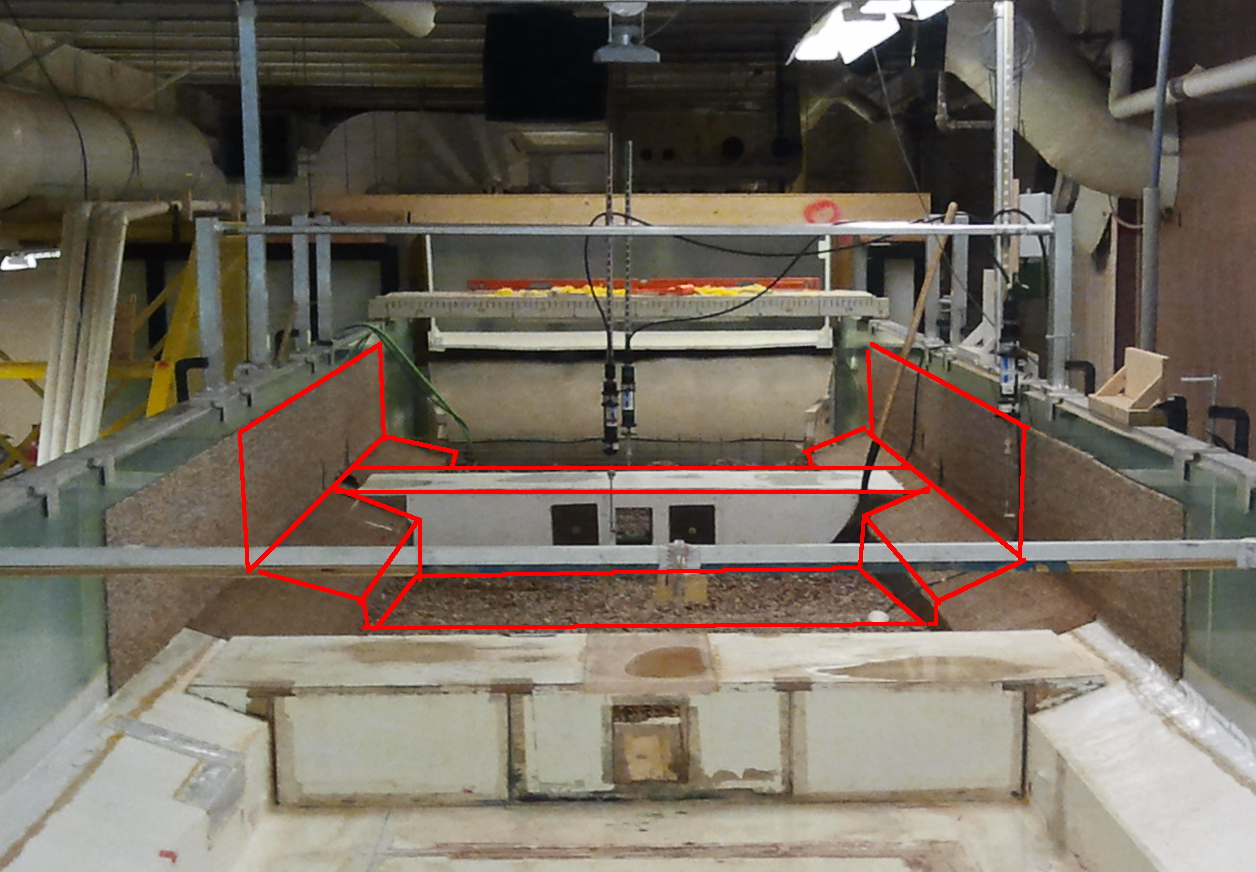
\includegraphics[width=5in]{researchflume.jpg} 
   \caption{Research flume looking upstream.  Red outline is approximate geometry of SToRM model application.  Culvert system was blocked, so that flow must pass over the inclusion in the channel.}
   \label{fig:ResearchFlume}
\end{figure}

The second case is a portion of the White River at US 82 near Crosbyton, Texas.   The study site is located proximal to US 82 and within the Texas Department of Transportation Silver Falls Rest Area.  Figure \ref{fig:WhiteRiverAerial} is a Google Earth base image, with author drawn lines to indicate the approximate study area (brown lines), the thalweg (cyan), and four cross sectional elevation survey trnasects.   Some additional elevations were collected.  A dam is located near the west-bound bridge of US 82 (depicted in the photograph as the double thick brown lines) .   Remnants of tropical system ``Alex'' in early July, 2010 provided rain in the region and the peak rainfall near the site occurred on July 4, 2010.   After this event, the second author performed a post-storm field survey using conventional USGS slope-area computations to estimate the peak discharge at the site from the debris lines left by the discharge, and an independent estimate of flow over the Silver Falls dam.  

\begin{figure}[h!] %  figure placement: here, top, bottom, or page
   \centering
   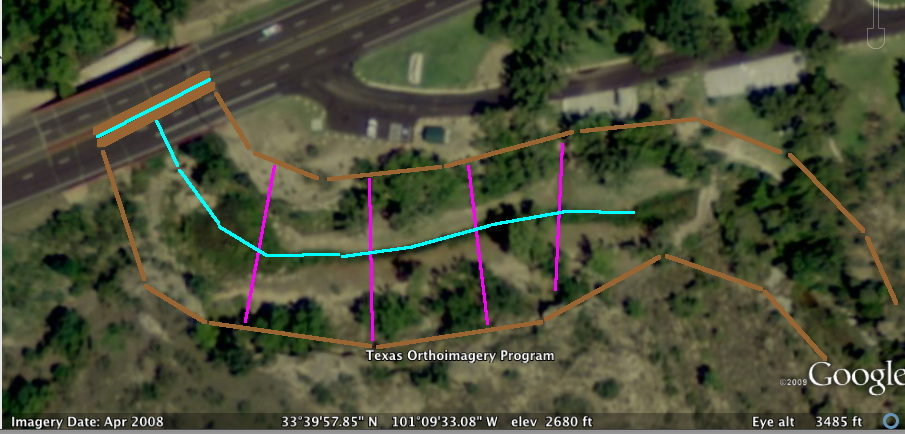
\includegraphics[width=5in]{WhiteRiverAerial.jpg} 
   \caption{Aerial view of White River case study.   Approximate location of thalweg, dam, and surveyed cross sections are indicated by the annotated segments.   Additional elevation locations are not depicted on the figure.  Flow is from left to right in this photograph.  Base image from \cite{GoogleEarth2011}.}
   \label{fig:WhiteRiverAerial}
\end{figure}
\clearpage
\section*{METHODS}

\subsection*{Developing Topographic Data for SToRM}
SToRM uses a topographic database in XYZ format.   In both case studies herein a Reflectorless Total Station was used to generate elevation survey data, and Surfer \citep{surfer2010} was used to generate an elevation grid before supplying the elevation information to the SToRM model.   The gridding algorithms that produced surfaces that ``looked'' most like the actual cases were kriging and nearest-neighbor interpolation.  Analyst intervention was used in a grid-node editor to force certain elevations to be faithful to actual elevations observed in the two case studies.

\subsubsection*{Topographic Model for the Research Flume}
The laboratory has 26 targets located around the interior of the building to allow the survey instrument to locate itself anywhere on or near the flume to allow for relatively high-resolution elevation surveys of the experimental bed and walls.   The use of a field instrument is by design --- the laboratory's purpose is to experiment with field-equivalent technologies.  An elevation survey was conducted in the laboratory flume using a subset of these targets to establish a coordinate system, and then a high-resolution survey (in excess of 200 locations on the flume floor, walls, and the culvert inclusion) was conducted.   These data were gridded using kriging in SURFER (using program defaults with analyst oversight to model the walls correct)\citep{dixon2011}.   This gridded data was then input into SToRM as the topographic survey.   

Figure \ref{fig:flume-elevation-image} is a plot of the elevation survey results, after processing, and rendered as a 3D surface.   This data arte then exported as XYZ ASCII and become input for SToRM.

\begin{figure}[htbp] %  figure placement: here, top, bottom, or page
   \centering
   \includegraphics[width=5in]{flume-elevation-image.jpg} 
   \caption{Research flume topographic database supplied to SToRM, looking upstream.  The survey data extended well beyond what is pictured and the sub-grid was simply clipped from the larger grid.}
   \label{fig:flume-elevation-image}
\end{figure}

Data from one of the archived experiments conducted with a blocked culvert system was selected from the data collection system.  That data contains water depths at ADV instrument locations, the location in XYZ of the ADV instrument measurement point, and the 3 components of the velocity field.   The data also contain the operational discharge of the particular experiment.  

\subsubsection*{Topographic Model for the White River}
The elevations obtained by the cross sections survey of the White River site were converted into a topographic grid for input to SToRM using the kriging algorithm in Surfer \citep{surfer2010} to generate a topographic model for importing into SToRM.   A boundary polygon that roughly follows the brown outline in Figure \ref{fig:WhiteRiverAerial} was then applied to force a physical boundary into the model.    Figure \ref{fig:white-river-elevation-image} is a plot of the elevation survey coordinates and the gridded data.   

The authors' found the gridding necessary because the TIN interoplator built into SToRM did not accomodate the comparatively acute angle in the lower left hand corner of the grid --- something humans can do quite without thinking was difficult for the algorithm to cope with.   A higher spatial density survey (as one would conduct if intentionally planning on using SToRM or similar tools) should eliminate the need for external gridding.   A weakness of the gridding exercise are the artifical pool sequence implied by the figure --- the authors' opinion is that the thalweg of the channel would join these ``pools'' and they are an artifact of the gridding algorithm.

\begin{figure}[htbp] %  figure placement: here, top, bottom, or page
   \centering
   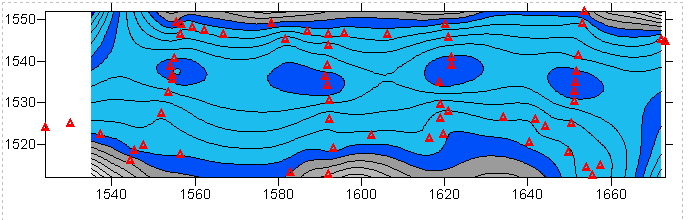
\includegraphics[width=6in]{white-river-elevation-image.jpg} 
   \caption{Contour map generated from gridded elevation survey.   Open triangles are locations of surveyed elevations in transformed XY coordinate system.}
   \label{fig:white-river-elevation-image}
\end{figure}

\subsection*{Resistance Model}
Both cases choose to use a Manning's-type resistance model for frictional effect in SToRM because of simplicity in input and because of the author's familarity with the Manning's loss model.  The program contains alternative and more recent model options.   In both cases a Manning's n value of 0.04 was selected as appropriate for the two cases.   Our opinion is that this numerical value is probably reasonable for the White River situation, and a bit too large for the laboratory situation.

\subsection*{Boundary, Initial and Simulation Control Conditions}
The simulation grid was built using program defaults as a starting point, then refining by trial-and-error until a grid of ``appropriate'' density was constructed.   The topography is then mapped to this grid.   The upstream boundary condition is a specified discharge that is distributed across a node string and presumably the program computes needed velocity.    The initial flow velocity was set as the inlet discharge divided by the outlet cross sectional flow area (a tyep of mean section velocity).  The initial conditions in both simulations were to set the water surface at the same depth as the downstream boundary condition.   

Selection of appropriate ``$\Delta~t$'' and several other simulation parameters was by trial-and-error.   One of the fundamental findings was that these values are not straightforward to specify a-priori, hence a substantially iterative simulation process is involved.   Once a small enough time step is found, then the simulations are run for substantial real time to produce a solution.   The data entry dialog box uses the description ``Courant Number'' where they seem to have meant ``Time-Step Length.''   This naming convention is only briefly mentioned in the tutorial and user manuals (which admittedly were works in-progress).  The internal (to the program) convergence plots do not necessarily mean the program has converged to an actual solution, but refers to an internal numerical consistency.   As non-CFD experts, this difference was discovered by considerable trial-and-error.

\section*{RESULTS}
The two cases were eventually simulated and a digest of results are presented.   The print media does not do justice to the program output, but will give a reader a flavor of the kind of results available.

\subsection*{Flume Velocities}
Figure \ref{fig:flume-simulation-image} is an annotated screen capture of the research flume simulation.   The three vertical red lines and red filled circles are the author's estimate of the location of ADV probes that were in the flow field during an actual experiment.   The discharge value in the experiment and the simulation is 0.56 m$^3$/s, with a downstream stage (left side of the simulation) of 4.01 m.   Table \ref{tab:flume-results} lists the simulated and measured velocities.   

% Requires the booktabs if the memoir class is not being used
\begin{table}[ht!]
   \centering
      \caption{Comparison of Measured and Simulated Velocities. 
      +X is to left, +Y is up in Figure \ref{fig:flume-simulation-image}}
   %\topcaption{Table captions are better up top} % requires the topcapt package
   \begin{tabular}{p{3in} p{0.6in} p{0.6in} p{0.6in} p{0.6in}}
   \hline
   Probe Location & V$_{x~meas.}$ & V$_{y~meas.}$ & V$_{x~mod.}$ & V$_{y~mod.}$ \\

   \hline
   \hline
   Upstream of Step (Rightmost Line) & 0.83 m/s & 0.03 m/s & 0.87 m/s & 0.03 m/s \\
   Downstream of Step (Middle Line) & 1.61 m/s & 0.06 m/s & 1.67 m/s & 0.02 m/s \\
   Further Downstream (Leftmost Line) & 0.72 m/s & 0.01 m/s & 0.94 m/s & 0.01 m/s \\
   \hline
   \hline
   \end{tabular}
\label{tab:flume-results}
\end{table}

\begin{figure}[h!] %  figure placement: here, top, bottom, or page
   \centering
   \includegraphics[width=6in]{flume-simulation-image.jpg} 
   \caption{Research flume flow field as simulated using SToRM.   The three filled circles represent approximate locations of 2D ADV instruments.}
   \label{fig:flume-simulation-image}
\end{figure}

The streamline field is representative of the appearance of the water surface in the experiment.  
There is a slight tilt to the flume longitudinal to the long axis that was detectable in the elevation surveys and with a spirit level.   
The fact that the numerical simulation is sensitive enough to this seemingly small asymmetry is astounding (to the authors) and the slight curvature in the simulated flow field is in the correct direction.  

The real flume is tilted slightly towards the bottom edge, and the magenta streamlines in Figure \ref{fig:flume-simulation-image} have some upward curvature as would be anticipated in such a tilt.   
The contraction of the streamlines is more pronounced in the numerical model than the actual model, but indeed in the real flume, flow is contracted over the inclusion.

Given the rather hasty nature of the SToRM modeling of the flume (experiments were ongoing and the opportunity to apply SToRM was an afterthought) the authors found the results reasonable.

\subsection*{White River Water Surface}
The White River study did not employ velocity measurements, so instead SToRM was evaluated in its ability to reproduce the observed water surface slope and other ancillary observations.   SToRM was run three times with the output from one run used as input for a subsequent run.   The time step increment was lengthened for each run, the idea was to get to an equilibrium solution.   After several million iterations the authors' decided that the program was as close to equilibrium as it was going to be for the purpose of this study (that is to evaluate the tool from a non-expert perspective).

\begin{figure}[htbp] %  figure placement: here, top, bottom, or page
   \centering
   \includegraphics[width=7in]{white-river-simulation-image.jpg} 
   \caption{Contour map generated from gridded elevation survey.   Open triangles are locations of surveyed elevations in transformed XY coordinate system.}
   \label{fig:white-river-simulation-image}
\end{figure}

Table \ref{tab:white-river-results} is a list of water surface elevations at the study site from the surveyed high water marks and from the simulation model.  The water surface slope as determined from field survey is about 0.0072 while the water surface slope computed by the model is about 0.0056.   Given the need to externally grid the topography and the gridding artifacts the authors' find these results reasonable.

\begin{table}[ht!]
   \centering
      \caption{Comparison of Measured and Simulated Water Surface Elevations}
   %\topcaption{Table captions are better up top} % requires the topcapt package
   \begin{tabular}{p{1in} p{1in} p{1in} p{1in} }
   Section & X Station (m)  & WSE$_{observed}$ & WSE$_{model}$  \\
   1 & 1554 & 27.52 & 27.58 \\
   2 & 1592 & 27.31 & 27.55 \\
   3 & 1618 & 27.04 & 27.43 \\
   4 & 1650 & 26.83 & 27.04 \\
   \end{tabular}
\label{tab:white-river-results}
\end{table}

\section*{CONCLUSIONS and DISCUSSION}
The results are meaningful in both case studies, but were more difficult to obtain that anticipated.   In the case of the research flume, the authors anticipated a more ``regular'' grid than the computer program generated --- this anticipation resulted in many hours expended to determine what was wrong (nothing but the author's expectations).   Selection of grid sizing is non-trivial, and the software defaults are simply starting points for the model users.   The SToRM documentation has some guidance, but other users need to consider this component of modeling an iterative step that will take considerable time.

Once a grid is selected that meets the user's needs, then the topography model needs to be mapped to that grid --- this mapping is neither automatic nor self-updating.   On many occasions the authors had to restart the entire modeling process because of the non-updating elevation map.   Rather then being a critique of the model, it is simply part of the protocol the user must remember.   The program authors left the program built in such a way that the difficult to build files (topography, etc.) are never destroyed, so restarts are not expensive in terms of time and effort.

The topographic description is an area of additional consideration.   The program is quite capable of producing output from a minimal topographic survey, but the meaning of such results is not clear.   We instead elected to use kriging and other algorithms to produce a topographic field that ``looked'' like the actual topography that was to be simulated.   This added effort is another area of modeling that may take considerable time.   The management of these data are not too difficult, but users are advised to maintain raw data copies in directories unrelated to SToRM in case they clobber a topography file.  The model and real coordinate systems in a practical application need far more advance consideration than that used in the case studies.  With modern towed ADV that can sound (determine depth) the high-spatial-resolution survey needed for the program to function well is realistic, and combined with an elevation survey of the land surface above the waterline, with some analyst guidance a dense survey like that implied by the ``gridded'' data sets is feasible and advised.

The steady flow simulation herein are in fact transient simulations to equilibrium.   The ``$\Delta$ t'' is adjusted in the simulation control portion of the program as a ``Courant Number'' and we found that by iteration a user could produce a result in a reasonable amount of perceived time.  We would start with a small value ($10^{-6}$) and instruct the program to run just a few iterations (10,000).   If the the model appeared stable, then we would increase the value, restart from the prior simulation, and run again for a few iterations (10,000).   This iterative process is repeated until the model fails, which it did spectacularly!   We would then return to the previous ``good" value and run many iterations ($\approx 10^{7}$).   During this iterative process, the convergence results reported by the program would be misleading --- again because the meaning of convergence for the model and the authors' was different.   The model appeared to be testing convergence of its computations within a time-step and not necessarily globally to the problem. 

Once we found an appropriate ``$\Delta$ t'', the model would be run sequentially several times, each time using the prior solution as the starting solution.   Eventually solutions stopped changing in variables of interest (at least to our satisfaction), and we took these soluton as the equilibrium conditions that represented a steady flow solution.    However, without external measurements with which to compare the simulation results, the authors' opinion is that a modeler would not know when a solution is adequate (at least for steady-flow).

The overriding lesson learned is the recognition that simulation convergence requires a different connotation from mass-balance convergence when using SToRM.  We were eventually able to mimic two observed cases, but with more effort than anticipated.   As an operational tool the authors would likely run conventional 1-D steady flow models to have a better grasp on the initial conditions to supply to the 2-D model.   The need for 2-D modeling would have to be established. 

The authors' use of SToRM allows us to use cross-sections that may not be perpendicular to the average flow field as assumed in 1-D models.  The ability to simulate flow in bends and around pier arrays is of further use, our interest is in recirculation, location of areas (plan view) where the discharge contribution is negligible, and similar questions.  If a situation needs 2-D modeling, SToRM is within the skill set of hydraulic modelers without CFD expertise, but a substantial learning effort is involved on the order of several weeks.   Furthermore, the use of external gridding software is likely to be required, so users will need that skill set.

\section*{ACKNOWLEDGEMENTS}
The simulations for the first two cases were conducted as part of a modeling seminar at Texas Tech University.  The author's are indebted to the other students in that seminar: John Dawley, Matthew Dirksen, Jeremy Dixon, Jeremy Kight, Travis Kaatz, Robert Pavur, Janice Rainwater, Brian Schuetze, and Vamshi Thummuri.  These students endured hours of the authors' reverse engineering of SToRM and individually ran versions of the models presented herein.   The ability to operate the tool was developed collectively in that modeling seminar.

The simulations for the last case were conducted by Janice Rainwater as part of her master's report; the conventional 1-D model uses to seed the program was built and run by Travis Kaatz.



\begin{thebibliography}{}

\bibitem[USGS, 2011]{storm2011}
{USGS Geomorphology Laboratory} (2011).
\newblock System for Transport and River Modeling.   \url{http://wwwbrr.cr.usgs.gov/projects/GEOMORPH_Lab/project-SToRM.html} Webpage last accessed, 12 Jan 2012.

\bibitem[McDonald and others, 2012]{mdswms2012}
{McDonald, R.R., Nelson, J.M., and Bennett, J.P.}, (2012).  \textsl{in press}. Multi-dimensional surface-water modeling system user�s guide: U.S. Geological Survey Techniques and Methods, 6-B2, 136 p.

\bibitem[Google Earth, 2011]{GoogleEarth2011}
{Google Earth, Google Inc.}, (2011). 
\url{http://www.google.com/earth/index.html} 
1600 Amphitheatre Parkway Mountain View, CA, 94043

\bibitem[Golden Software, 2010]{surfer2010}
{Golden Software, Inc.}, (2010). Surfer 10.
809 14th Street, Golden, Colorado 80401-1866, U.S.A.
Phone: 303-279-1021 Fax: 303-279-0909
\url{www.GoldenSoftware.com}

\bibitem[Dixon, J. 2011]{dixon2011}
{Dixon, J.}, (2011). 
A Relation Between Select Hydraulic Properties and Sediment
Transport Volume Through Experimental Culvert Configurations
and Techniques for Measuring Sediment Transport Volumes.
MS Thesis, Department of Civil and Environmental Engineering, Texas Tech University, 117 p.

\end{thebibliography}

\end{document}


% eof